\section{Graphs}

In Königsberg in Prussia, there is an island connected
with bridges to the banks of a river.

\begin{figure}
    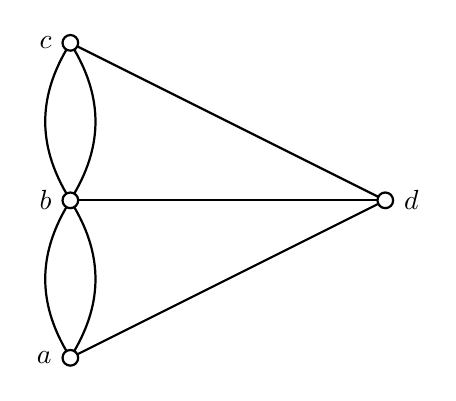
\begin{tikzpicture}[thick, main/.style = {draw, circle}]
        \node[main,scale=0.6, label=left:$a$] (a) at (0,0) {};
        \node[main,scale=0.6, label=left:$b$] (b) at (0,2) {};
        \node[main,scale=0.6, label=left:$c$] (c) at (0,4) {};
        \node[main,scale=0.6, label=right:$d$] (d) at (4,2) {};

        \draw (a) -- (d);
        \draw (b) -- (d);
        \draw (c) -- (d);
        \draw (a) to [out=120,in=240,looseness=1] (b);
        \draw (a) to [out=60,in=300,looseness=1] (b);

        \draw (b) to [out=120,in=240,looseness=1] (c);
        \draw (b) to [out=60,in=300,looseness=1] (c);

    \end{tikzpicture}
    \caption{The Seven Bridges of Königsberg}
\end{figure}

It was asked whether anyone could arrange a route in
such a way that he could cross each bridge once and
only once. Euler modelled the island and banks as
\emph{nodes}. Formally, this question asks if there is a cyclic
path that uses each edge once and only once. It turns out
there is provided the graph is connected and all nodes have
even degree.

Some terminology:

\begin{itemize}
    \item \textbf{Node}: Also known as points or vertices. Fundemental
          building block of a graph.
    \item \textbf{Edge}: Connects two nodes, or a node to itself.
    \item \textbf{Walk}: A sequence of vertices and edges, where the edges connect the adjacent vertices in the sequence.
    \item \textbf{Tour}: A walk with no repeated edges.
    \item \textbf{Path}: A walk with no repeated vertices. A \emph{simple} path has no repeated nodes.
    \item \textbf{Adjacent}: Said of two nodes connected by an undirected edge,
          or of the node to which a directed edges enters and the node of the edge's origin.
    \item \textbf{Degree}: Number of edges going out from a node. In a directed graph,
          there are both in and out degrees.
    \item \textbf{Cycle}: A path from a node to itself. If there is a cycle in a
          graph, it is a cyclic graph. Else it is acyclic.
    \item \textbf{Connected}: An undirected graph is connected if every node can be reached
          from every other node. For a directed graph, the same property is called strongly connected.
\end{itemize}

Some notation: an undirected graph $G(V,E)$ consists of a set of nodes $V$
and edges $E$. Perhaps $V = {A, B, C}$ and $E = {(A,B), (A,A), (A, C)}$.
A directed graph $G<V, E>$ might have the same vertices, but edges
$E = {<A,B>, <A,A>, <A, C>}$ indicating that one may only travel from $A$
to other nodes.

There are two kinds of graph, \emph{directed} and \emph{undirected}.
In an undirected graph like the one shown previously, an edge can
go both ways. In a directed graph one can travel only one way along an
edge, represented by an arrow like in figure \ref{fig:directedgraph}

\begin{figure}
    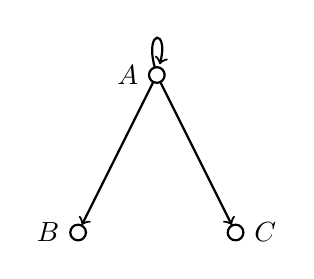
\begin{tikzpicture}[thick, main/.style = {draw, circle}]
        \node[main,scale=0.6, label=left:$A$] (a) at (0,2) {};
        \node[main,scale=0.6, label=left:$B$] (b) at (-1,0) {};
        \node[main,scale=0.6, label=right:$C$] (c) at (1,0) {};

        \draw[->] (a) -- (b);
        \path[->] (a) edge [loop above] ();
        \draw[->] (a) -- (c);

    \end{tikzpicture}
    \caption{Example of a Directed Graph}
    \label{fig:directedgraph}
\end{figure}

A \emph{weighted} graph has weights assocted with each directed edge. The weight
could represent probability of moving from one node to another, travel times, distances,
etc.